\begin{problem}{관광 사업}{표준 입력(stdin)}{표준 출력(stdout)}{5\,초}{1024\,MB}

옥토끼나라는 $N$개의 도시를 잇는 $N-1$개의 도로로 이루어진 나라다. 어떤 도시에서도 원하는 다른 도시로 도로만을 통해 이동할 수 있다. 즉, 옥토끼나라는 트리 구조를 이룬다. 각 도로는 자연수 길이를 가지고 있으며, 두 도시 간의 거리는 두 도시를 잇는 단순 경로 위의 도로의 길이의 합이다.

옥토끼나라의 새로운 관광 사업으로 두 도시 $X$와 $Y$를 골라, 두 도시간에 관광 자매결연 관계를 맺을 것이다. 자매결연을 맺으면 두 도시의 사람들이 서로 관광을 하기 위해 이동할 것이다. 그렇기에 $D\left(X,Y\right)$를 $X$와 $Y$ 사이의 거리, $C_X$와 $C_Y$를 각각 $X$와 $Y$에 거주하는 인구 수라고 하면 교통료로 $\left(C_X+C_Y\right) \times D\left(X,Y\right)$의 수익을 얻을 수 있다.

옥토끼나라는 요즘 격변을 겪고 있어 도시의 인구 수가 계속 바뀌고, 자매결연 계획에 참가하려는 도시들도 상황에 따라 다양하기 때문에 다양한 상황에서 자매결연 관계를 맺을 도시들을 구해야 한다.

$Q$개의 자매결연 계획이 주어진다. 각 계획은 $X$의 후보 도시 의 집합 $A$, $Y$의 후보 도시의 집합 $B$가 주어지며, 각 후보 도시의 인구 수 $C_u$가 주어진다. $A$와 $B$에 동시에 포함되는 도시는 없다.

각 자매결연 계획마다, $X$와 $Y$를 정해서 얻을 수 있는 최대의 교통료 수익을 구해야 한다.

\InputFile
첫 줄에 $N$과 $Q$가 공백으로 구분되어 주어진다. ($1 \leq N \leq 300\ 000$, $1 \leq Q \leq 100\ 000$)

그 다음 $N-1$개의 줄에 걸쳐 도로의 정보 $u$, $v$, $d$가 공백으로 구분되어 주어진다. 이는 $i$번째 도로가 도시 $u$와 도시 $v$를 이으며 길이는 $d$라는 뜻이다. ($1 \leq u,v \leq N$, $1 \leq d \leq 30$)

이후 $Q$개의 자매결연 계획이 다음과 같은 형식으로 주어진다.
\begin{itemize}
    \item 첫 줄에 $N_A$와 $N_B$가 공백으로 구분되어 주어진다. $N_A$는 $A$의 크기, $N_B$는 $B$의 크기다. ($1 \leq N_A,N_B, N_A+N_B \leq N$)
    \item 이후 $N_A$개의 줄에 걸쳐 $u$와 $p$가 공백으로 구분되어 주어진다. 이는 도시 $u$가 집합 $A$에 속하며 거주하는 인구 수가 $p$명, 즉 $C_u=p$라는 뜻이다. ($1 \leq u \leq N$, $1 \leq p \leq 3 \times 10^6$)
    \item 이후 $N_B$개의 줄에 걸쳐 $v$와 $q$가 공백으로 구분되어 주어진다. 이는 도시 $v$가 집합 $B$에 속하며 거주하는 인구 수가 $q$명, 즉 $C_v=q$라는 뜻이다. ($1 \leq v \leq N$, $1 \leq q \leq 3 \times 10^6$)
\end{itemize}

$\sum_{i=1}^{Q} (N_A+N_B)$는 $200\ 000$ 이하다.

\OutputFile
한 줄에 하나씩 순서대로 각 자매결연 계획의 최대 교통료 수익을 출력한다.

\Examples

\begin{example}
\exmp{
3 3
1 2 1
2 3 1
1 2
1 1
2 2
3 3
1 2
2 2
1 1
3 3
1 2
3 3
1 1
2 2
}{%
8
5
8
}%
\exmp{
7 1
1 2 10
3 4 1
4 5 1
2 4 6
4 6 6
6 7 10
3 3
1 1
2 3
3 5
5 5
6 3
7 1
}{%
102
}%
\end{example}
\Note
\begin{center}
    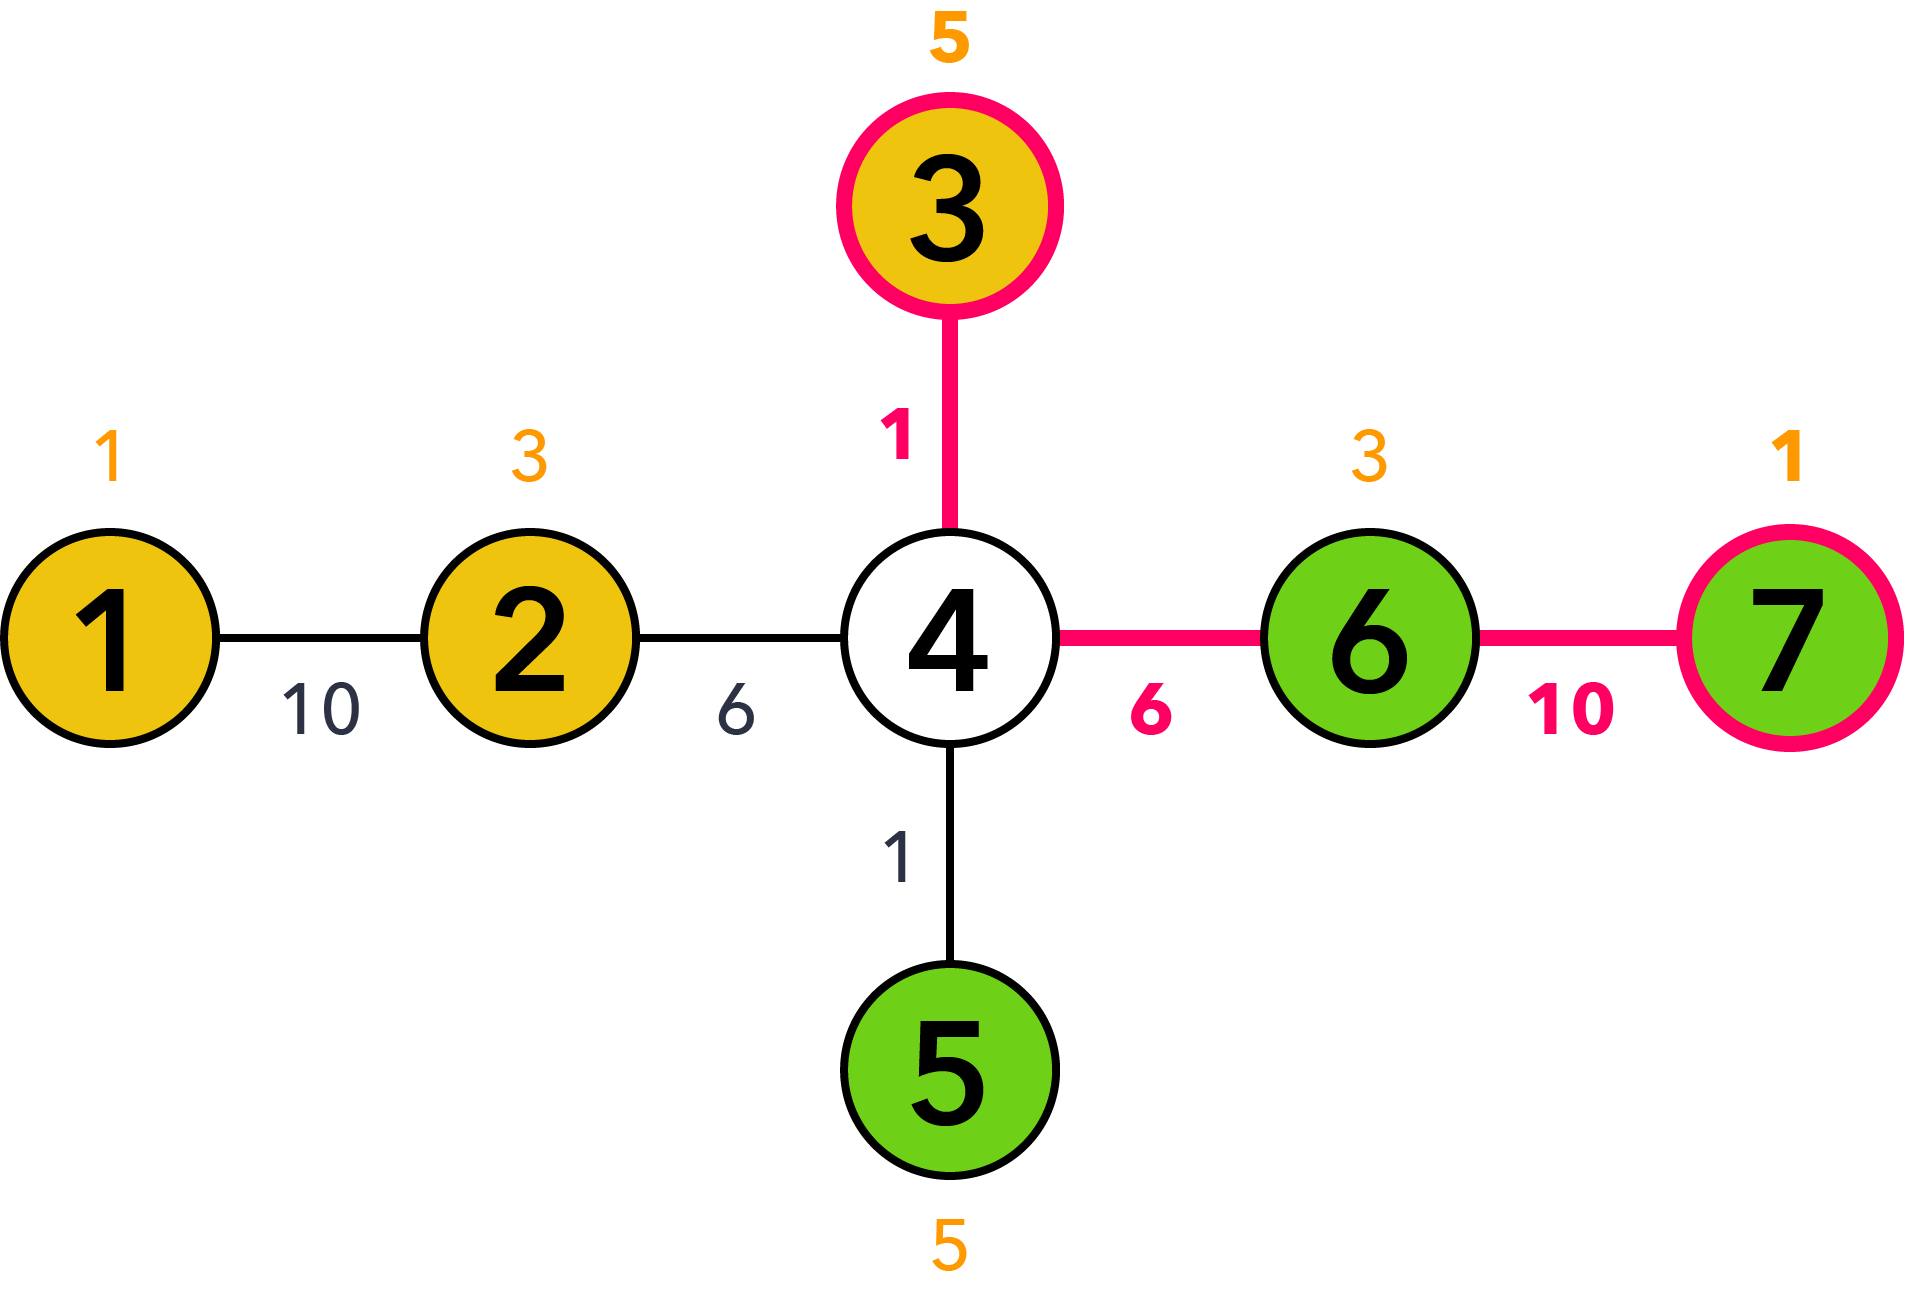
\includegraphics[width=.525\textwidth]{../pictures/tour@4x.png}
\end{center}
\textbf{예제 2}에서, $X=3$이고 $Y=7$인 경우 교통료 수익이 $(5+1) \times 17=102$로 최적이다. $X=1$이고 $Y=5$인 경우 또한 최적이다.
\end{problem}